\textbf{Contributions}

The material in this chapter expands on work presented in

~\autocite{cassellaExactChiralAmorphous2022} Cassella, G., D'Ornellas, P., Hodson, T., Natori, W. M., \& Knolle, J. (2022). An exact chiral amorphous spin liquid. \emph{arXiv preprint arXiv:2208.08246.}

the code is available at~\autocite{hodsonKoalaKitaevAmorphous2022}.

This was a joint project of Gino, Peru and myself with advice and guidance from Willian and Johannes (all authors of the above). The project grew out of an interest the three of us had in studying amorphous systems, coupled with Johannes' expertise on the Kitaev model. The idea to use Voronoi partitions came from~\autocite{marsalTopologicalWeaireThorpe2020} and Gino did the implementation of this. The idea and implementation of the edge colouring using SAT solvers, the mapping from flux sector to bond sector using A* search were both entirely my work. Peru produced the numerical evidence for the ground state and implemented the local markers. Gino and I did much of the rest of the programming for Koala while pair programming and 'whiteboard'ing, this included the phase diagram, edge mode and finite temperature analyses as well as the derivation of the projector in the amorphous case.

\hypertarget{amk-Model}{%
\section{The Model}\label{amk-Model}}

Already at with its introduction it was known that Kitaev honeycomb model would remain solvable on any three-coordinated \(z=3\) graph. Generalisation have been made to many lattices~\autocite{eschmannThermodynamicClassificationThreedimensional2020,Yao2009,eschmann2019thermodynamics,Peri2020} but so far none have fully broken the translation symmetry of the model by putting it onto a fully amorphous lattice.

Amorphous lattices are characterised by local constraints but no long range order. These arise, for instance, in amorphous semiconductors~like Silicon and Germanium~\autocite{Yonezawa1983,zallen2008physics}. Recent work has shown that topological insulating (TI) phases, characterized by protected edge states and topological bulk invariants, can exist in amorphous systems~\autocite{mitchellAmorphousTopologicalInsulators2018,agarwala2019topological,marsalTopologicalWeaireThorpeModels2020,costa2019toward,agarwala2020higher,spring2021amorphous,corbae2019evidence}. TI phases, however, arise in non-interacting systems. In this context, we might ask whether QSL systems and the KH model in particular could be realised on amorphous lattices. The phases of the KH model have many similarities with TIs but differ in that the KH model is an interacting system. In general, research on amorphous electronic systems has been focused mainly on non-interacting systems with the exception of amorphous superconductivity~\autocite{buckel1954einfluss,mcmillan1981electron,meisel1981eliashberg,bergmann1976amorphous,mannaNoncrystallineTopologicalSuperconductors2022} or very recent work looking to understand the effect of strong electron repulsion in TIs~\autocite{kim2022fractionalization}.

Looking more towards the KH model, magnetism in amorphous systems has been investigated since the 1960s, mostly through the adaptation of theoretical tools developed for disordered systems~\autocite{aharony1975critical,Petrakovski1981,kaneyoshi1992introduction,Kaneyoshi2018}. We have already seen that the topological disorder of amorphous lattices can be qualitatively different from standard bond or site disorder, especially in two dimensions~\autocite{barghathiPhaseTransitionsRandom2014,schrauthViolationHarrisBarghathiVojtaCriterion2018}. Research focused on classical Heisenberg and Ising models has accounted for the observed behaviour of ferromagnetism, disordered antiferromagnetism and widely observed spin glass behaviour~\autocite{coey1978amorphous}. However, the role of the spin-anisotropic interactions and quantum effects that we see in the KH model has not been addressed in amorphous magnets. It is an open question whether frustrated magnetic interactions on amorphous lattices can give rise genuine quantum phases such as QSLs~\autocite{Anderson1973,Knolle2019,Savary2016,Lacroix2011}. This chapter will answer that question positively by demonstrating that the Kitaev model on amorphous lattices leads to a kind of QSL called a chiral spin liquid (CSL).

In this section I will discuss how to generalise the Kitaev model to an amorphous lattice. The methods section discusses how to generate such lattices using Voronoi partitions of the plane~\autocite{mitchellAmorphousTopologicalInsulators2018,marsalTopologicalWeaireThorpeModels2020}, colour them using a SAT solver and how to map back and forth between gauge field configurations and flux configurations. In the results section, I will show extensive numerical evidence that the model follows the simple generalisation to Lieb's theorem~\autocite{lieb_flux_1994} found by other works~\autocite{eschmannThermodynamicClassificationThreedimensional2020,Yao2009,eschmann2019thermodynamics,Peri2020}. I then map out the phase diagram of the model and show that the chiral phase around the symmetric point (\(J_x = J_y = J_z\)) is gapped and characterized by a quantized local Chern number \(\nu\)~\autocite{peru_preprint,mitchellAmorphousTopologicalInsulators2018} as well as protected chiral Majorana edge modes. Finally, I look at the role of finite temperature fluctuations and show that the proliferation of flux excitations leads to an Anderson transition similar to that of the Falicov-Kimball model, to a thermal metal phase~\autocite{Laumann2012,lahtinenTopologicalLiquidNucleation2012,selfThermallyInducedMetallic2019}. Finally I consider possible physical realisations of this model and the motivations for doing so.

\hypertarget{fig:amk-zoom}{%
\begin{figure}
\centering
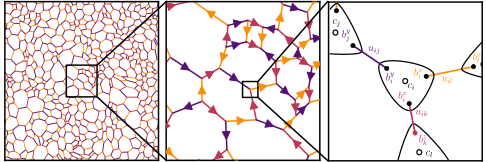
\includegraphics[width=1\textwidth,height=\textheight]{figure_code/amk_chapter/intro/amk_zoom/amk_zoom_by_hand}
\caption[{The Kitaev Honeycomb Model}]{\textbf{(a)} The standard Kitaev model is defined on a honeycomb lattice. The special feature of the honeycomb lattice that makes the model solvable is that each vertex is joined by exactly three bonds, i.e.~the lattice is trivalent. One of three labels is assigned to each \textbf{(b)}. We represent the antisymmetric gauge degree of freedom \(u_{jk} = \pm 1\) with arrows that point in the direction \(u_{jk} = +1\) \textbf{(c)}. The Majorana transformation can be visualised as breaking each spin into four Majoranas which then pair along the bonds. The pairs of x,y and z Majoranas become part of the classical \(\mathbb{Z}_2\) gauge field \(u_{ij}\). This leaves a single Majorana \(c_i\) per site.}
\label{fig:amk-zoom}
\end{figure}
}

As Kitaev pointed out in his original paper introducing the KH model, it remains solvable on any lattice which satisfies two properties. First the lattice must first be trivalent, that is, every vertex must three edges attached to it~\autocite{kitaevAnyonsExactlySolved2006,Nussinov2009}.

A well studied class of amorphous trivalent lattices are the 2D Voronoi lattices~\autocite{mitchellAmorphousTopologicalInsulators2018,florescu_designer_2009,marsalTopologicalWeaireThorpeModels2020}. These arise from Voronoi partitions of the plane. Given a set of seed points, the Voronoi partition divides the plane into regions based on which seed point is closest. The `spheres of influence' of each seed point form the plaquettes of the resulting lattices, while the boundaries become the edges. The Voronoi partition exists in arbitrary dimensions and produces lattices with coordination number \(d+1\) except for degenerate cases with measure zero~\autocite{voronoiNouvellesApplicationsParamètres1908,watsonComputingNdimensionalDelaunay1981}. Hence this Voronoi partitions in two dimensions lends themselves natural to the Kitaev model.

Other methods of lattice generation are possible, one can connect randomly placed sites based on proximity~\autocite{agarwala2019topological} or create simplices from random sites~\autocite{christRandomLatticeField1982}. However these methods do not present a natural way to restrict the vertex degree to a constant. Perhaps ideally, we would sample uniformly from the space of possible trivalent graphs, there has been some work on how to do this using a Markov Chain Monte Carlo approach~\autocite{alyamiUniformSamplingDirected2016}. However, it does not guarantee that the resulting graph is planar, which is necessary to be able to 3-edge-colour the lattice, our second constraint.

The second constraint required for the Kitaev model to remain solvable is that we must be able to assign labels to each bond \(\{x,y,z\}\) such that each no two edges of the same label meet at a vertex. Such an assignment is is known as a 3-edge-colouring. For translation invariant models we need only find a solution for the unit cell which is usually small enough that this can be done by hand. The difficulty is compounded by the fact that, to the best of my knowledge, the problem of edge-colouring is NP-Hard. To find colourings in practice, we will employ a standard method from the computer science literature for finding solutions of NP-Hard problems called a SAT solver, this is discussed in more detail in the \protect\hyperlink{amk-methods}{methods secton}.

We find that for larger lattices there are in general many valid colourings. In the isotropic case \(J^\alpha = 1\) the colouring has no physical significance. As the definition of the four Majoranas at a site is arbitrary, we can define a local operator that transforms the colouring of any particular site to another permutation and show that these operators commute with the Hamiltonian. We cannot do this in the anisotropic case but we nevertheless expect the lattices to exhibit a self averaging behaviour in larger systems when the colouring is chosen arbitrarily.

\hypertarget{fig:state_decomposition_animated}{%
\begin{figure}
\centering
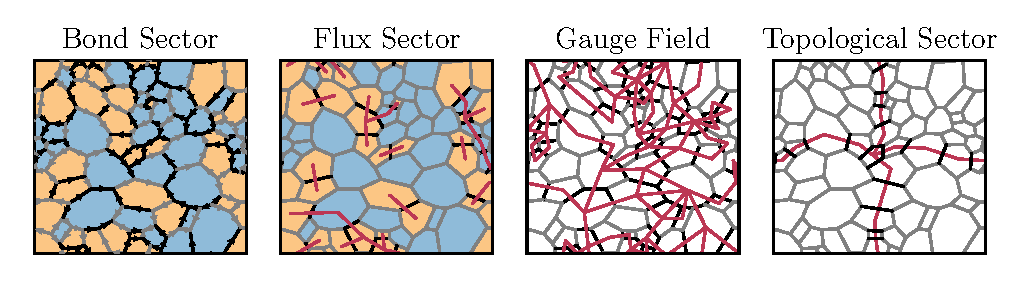
\includegraphics[width=1\textwidth,height=\textheight]{figure_code/amk_chapter/intro/state_decomposition_animated/state_decomposition_animated}
\caption[{State Decomposition}]{(Bond Sector) A state in the bond sector is specified by assigning \(\pm 1\) to each edge of the lattice. However, this description has a substantial gauge degeneracy. We can simplify things by decomposing each state into the product of three kinds of objects: (Vortex Sector) Only a small number of bonds need to be flipped (compared to some arbitrary reference) to reconstruct the vortex sector. Here, the edges are chosen from a spanning tree of the dual lattice, so there are no loops. (Gauge Field) The `loopiness' of the bond sector can be factored out. This gives a network of loops that can always be written as a product of the gauge operators \(D_j\). (Topological Sector) Finally, there are two loops that have no effect on the vortex sector, nor can they be constructed from gauge symmetries. These can be thought of as two fluxes \(\Phi_{x/y}\) that thread through the major and minor axes of the torus. Measuring \(\Phi_{x/y}\) amounts to constructing Wilson loops around the axes of the torus. We can flip the value of \(\Phi_{x}\) by transporting a vortex pair around the torus in the \(y\) direction, as shown here. In each of the three figures on the right, black bonds correspond to those that must be flipped. Composing the three together gives back the original bond sector on the left. \href{http://thomashodson.com/assets/thesis/figure_code/amk_chapter/intro/state_decomposition_animated/state_decomposition_animated.gif}{ Animated version online.}}
\label{fig:state_decomposition_animated}
\end{figure}
}

On a lattice with the above properties, the solution laid out in~\protect\hyperlink{bg-hkm-model}{the kitaev model} remains applicable to our Amorphous Kitaev (AK) model, see \cref{fig:amk-zoom} for an example lattice generated by our method. The main differences are twofold. Firstly, the lattices are no longer bipartite in general and therefore contain plaquettes with an odd number of sides which have flux \(\pm i\). This leads the AK model to have a ground state with spontaneously broken chiral symmetry~\autocite{Chua2011,yaoExactChiralSpin2007,ChuaPRB2011,Fiete2012,Natori2016,Wu2009,Peri2020,WangHaoranPRB2021}. This is also similar to the behaviour of the original Kitaev model in response to a magnetic field. One ground state is related to the other by globally inverting the imaginary \(\phi\) fluxes~\autocite{yaoExactChiralSpin2007}.

Secondly, as the model is no longer translationally invariant, Lieb's theorem for the ground state flux sector no longer applies. However as discussed in the background, a simple generalisation of Lieb's theorem has been shown numerically to be applicable to many generalised Kitaev models~\autocite{eschmannThermodynamicClassificationThreedimensional2020,Yao2009,eschmann2019thermodynamics,Peri2020}. This generalisation states that the ground state flux configuration depends on on the number of sides of each plaquette \(\phi = -(\pm i)^{n_{\mathrm{sides}}}\) with a twofold global chiral degeneracy.

The obvious approach would be to verify that this generalises to the AK model numerically via exhaustive checking of flux configurations. However this is problematic because the number of states to check scales exponentially with system size. We side step this by gluing together two methods, we first work with lattices small enough that we can fully enumerate their flux sectors but tile them to reduce finite size effects. We then show that the effect of tiling scales away with system size.

\hypertarget{fig:majorana_bound_states}{%
\begin{figure}
\centering
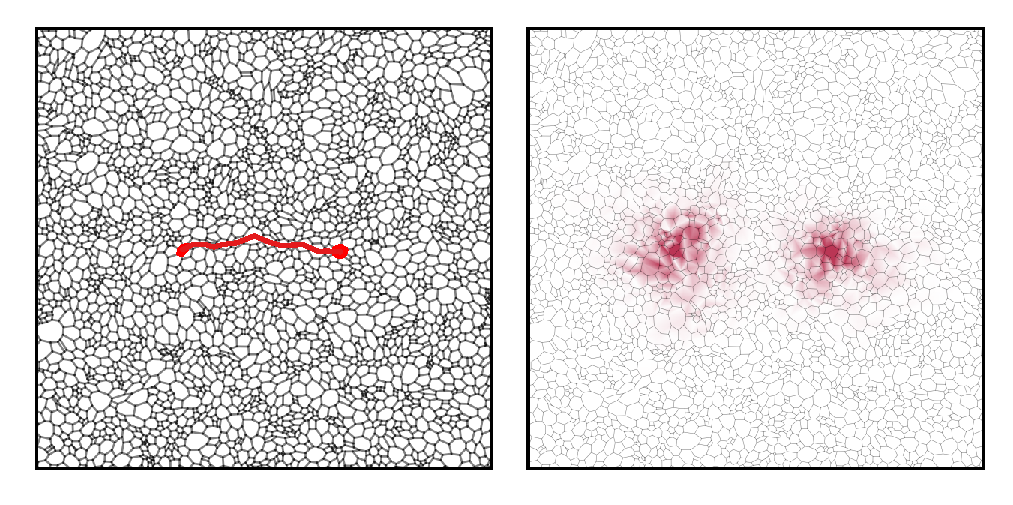
\includegraphics[width=1\textwidth,height=\textheight]{figure_code/amk_chapter/majorana_bound_states/majorana_bound_states}
\caption[{Majorana Bound States}]{(Left) A large amorphous lattice in the ground state save for a single pair of vortices shown in red, separated by the string of bonds that we flipped to create them. (Right) The density of the lowest energy Majorana state in this vortex sector. These Majorana states are bound to the vortices. They `dress' the vortices to create a composite object.}
\label{fig:majorana_bound_states}
\end{figure}
}

In order to evaluate the Chern marker later, we need a way to evaluate the model on open boundary conditions. Simply removing bonds from the lattice leaves behind unpaired \(b^\alpha\) operators that must be paired in some way to arrive at fermionic modes. To fix a pairing, we always start from a lattice defined on the torus and generate a lattice with open boundary conditions by defining the bond coupling \(J^{\alpha}_{ij} = 0\) for sites joined by bonds \((i,j)\) that we want to remove. This creates fermionic zero modes \(u_{ij}\) associated with these cut bonds which we set to 1 when calculating the projector. Alternatively, since all the fermionic zero modes are degenerate anyway, an arbitrary pairing of the unpaired \(b^\alpha\) operators could be performed.

\hypertarget{the-euler-equation}{%
\subsection{The Euler Equation}\label{the-euler-equation}}

Euler's equation provides a convenient way to understand how the states of the AK model factorise. The Euler equation states if we embed a lattice with \(B\) bonds, \(P\) plaquettes and \(V\) vertices onto a closed surface of genus \(g\), (\(0\) for the sphere, \(1\) for the torus) then

\[B = P + V + 2 - 2g\]

For the case of the torus where \(g = 1\), we can rearrange this and exponentiate it to read:

\[2^B = 2^{P-1}\cdot 2^{V-1} \cdot 2^2\]

This corresponds to the fact that their are \(2^N\) configurations of the bond variables \(\{u_{ij}\}\), each of these configurations can be uniquely decomposed into a flux sector, a gauge sector and a topological sector, see \cref{fig:state_decomposition_animated}. Each of the \(P\) plaquette operators \(\phi_i\) takes two values but vortices are created in pairs so there are \(2^{P-1}\) vortex sectors in total. There are \(2^{V-1}\) gauge symmetries formed from the \(V\) symmetry operators \(D_i\) because \(\prod_{j} D_j = \mathbb{1}\) is enforced by the projector. Finally, the two topological fluxes \(\Phi_x\) and \(\Phi_y\) account for the last factor \(2^2\).

In addition, The fact that we only work with trivalent lattices implies that each vertex shares three bonds with other vertices so effectively comes with \(\tfrac{3}{2}\) bonds. This is consistent with the fact that, in the Majorana representation on the torus, each vertex brings three \(b^\alpha\) operators which then pair along bonds to give \(3/2\) bonds per vertex. Substituting \(3V = 2B\) into Euler's equation tells us that any trivalent lattice on the torus with \(N\) plaquettes as \(2N\) vertices and \(3N\) bonds. Since each bond is part of two plaquettes this implies that the average mean number of sides of a plaquette is exactly six and that odd sides plaquettes must come in pairs.
